\section{Model and Design}
\label{sec:model}


A workflow is modeled as a Directed Acyclic Graph (DAG). Each node in the DAG often represents a workflow task ($t$), and the edges represent dependencies between the tasks that constrain the order in which tasks are executed. Dependencies typically represent data-flow dependencies in the application, where the output files produced by one task are used as inputs of another task. Each task is a program and a set of parameters that need to be executed. Fig.~\ref{fig:model_odag} (left) shows an illustration of a DAG composed by four tasks. This model fits several workflow management systems such as Pegasus~\cite{Deelman:2005:PFM:1239649.1239653}, Askalon~\cite{Fahringer:2005:ATS:1064323.1064331}, and Taverna~\cite{Oinn:2006:TLC:1148437.1148448}. 

\begin{figure}[htb]
	\centering
	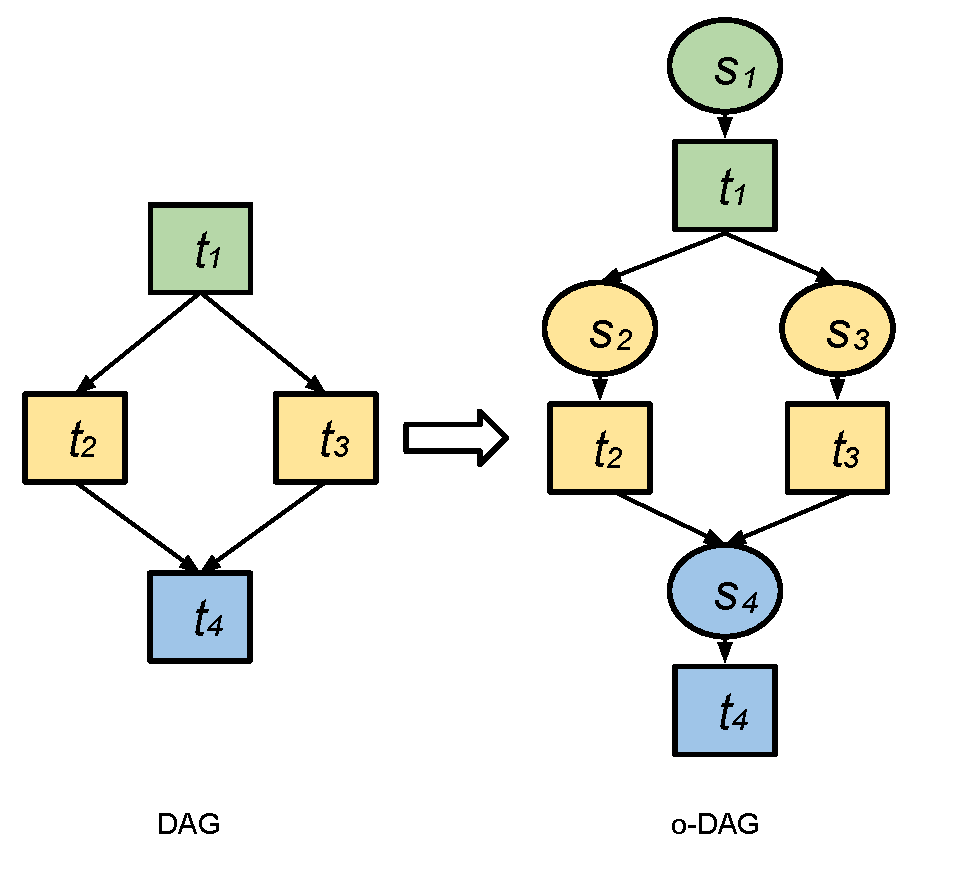
\includegraphics[width=0.7\linewidth]{figures/model/odag_color.pdf}
	\captionof{figure}{Extending DAG to o-DAG.}
	\label{fig:model_odag}
	\vspace{-15pt}
\end{figure}

%I may need to keep them here since I need to introduce the o-DAG model and it is execution dependent. 
Fig.~\ref{fig:model_system} shows a typical workflow execution environment. The submit host prepares a workflow for execution (clustering, mapping, etc.), and worker nodes, at an execution site, execute jobs individually. The main components are introduced below:

\begin{figure}[htb]
\centering
  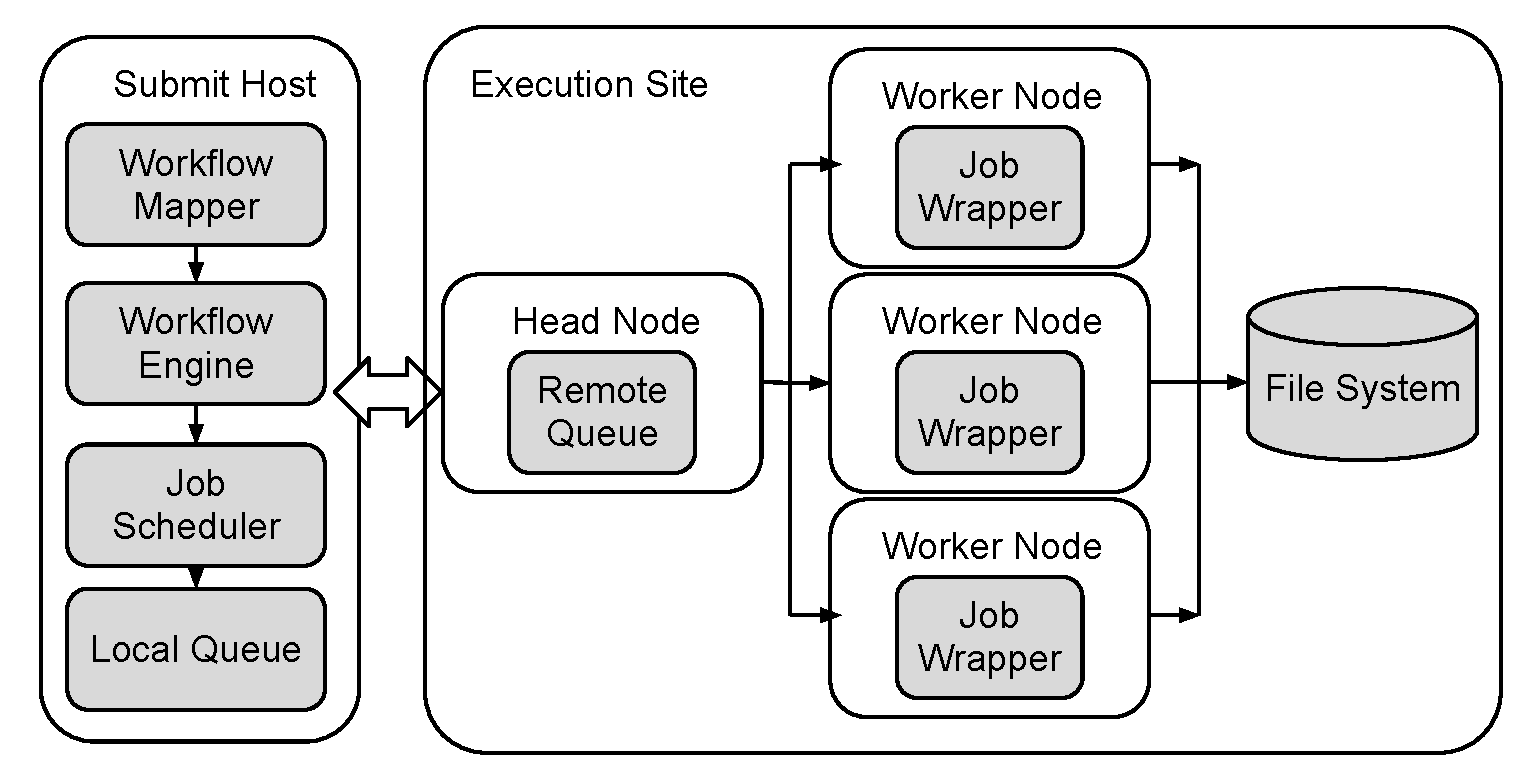
\includegraphics[width=0.95\linewidth]{figures/model/execution.pdf}
  \caption{A workflow system model.}
  \label{fig:model_system}
  \vspace{-15pt}
\end{figure}

\begin{figure}[!htb]
\centering
 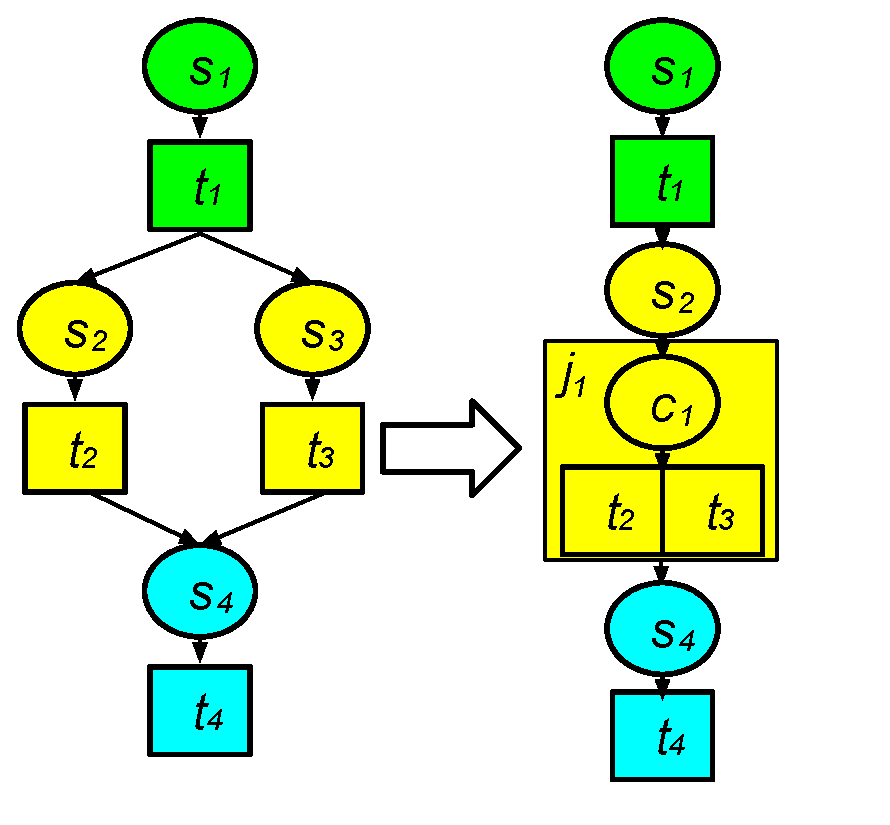
\includegraphics[width=0.65\linewidth]{figures/model/hc_color.pdf}
  \captionof{figure}{An Example of Horizontal Clustering. (Color indicates the horizontal level of a task)}
  \label{fig:model_hc}
  \vspace{-15pt}
\end{figure}

\begin{figure}[!htb]
\centering
 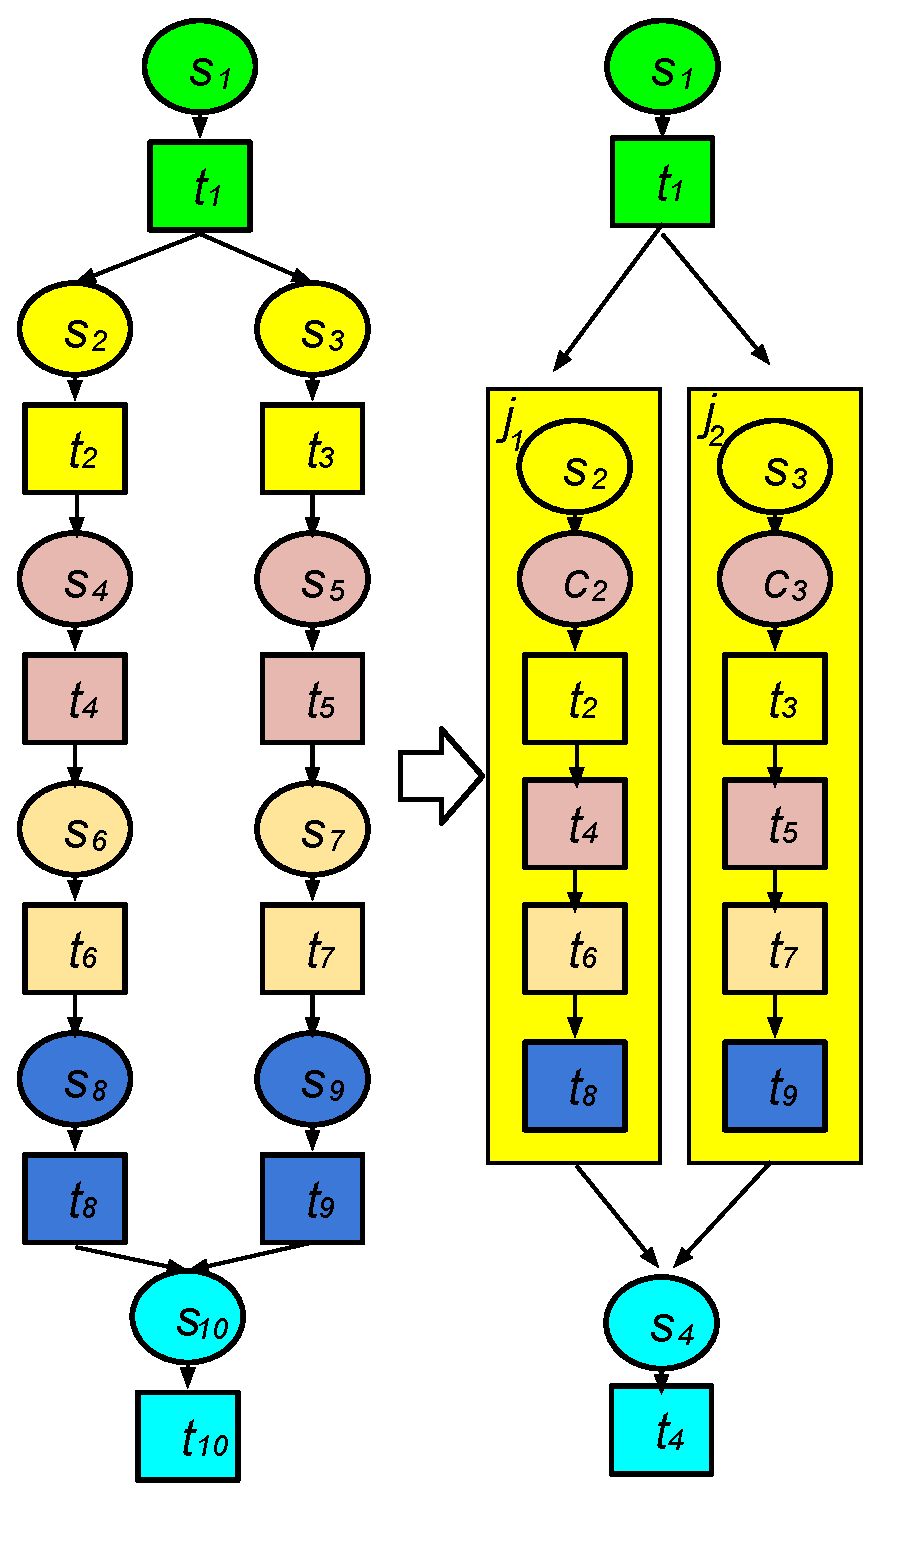
\includegraphics[width=0.65\linewidth]{figures/model/vc_color.pdf}
  \captionof{figure}{An Example of Vertical Clustering.}
  \label{fig:model_vc}
  \vspace{-15pt}
\end{figure}

\paragraph{Workflow Mapper} generates an executable workflow based on an abstract workflow provided by the user or workflow composition system. It also restructures the workflow to optimize performance and adds tasks for data management and provenance information generation. In this work, the workflow mapper is used to merge small tasks together into a job such that system overheads are reduced. This is called \textbf{Task Clustering}. A job is a single execution unit in the workflow execution systems and may contain one or more tasks. 


\paragraph{Workflow Engine} executes jobs defined by the workflow in order of their dependencies. Only jobs that have all their parent jobs completed are submitted to the Job Scheduler. The Workflow Engine relies on the resources (compute, storage, and network) defined in the executable workflow to perform the necessary actions. The time period when a job is free (all of its parents have completed successfully) to when it is submitted to the job scheduler is denoted the workflow engine delay. The workflow engine delay is usually configured by users to assure that the entire workflow scheduling and execution system is not overloaded. 

\paragraph{Job Scheduler and Local Queue} manage individual workflow jobs and supervise their execution on local and remote resources. The time period when a task is submitted to the job scheduler to when it starts its execution in a worker node is denoted as the queue delay. It reflects both the efficiency of the job scheduler and the resource availability. 

\paragraph{Job Wrapper} extracts tasks from clustered jobs and executes them at the worker nodes. The clustering delay is the  elapsed time of the extraction process.

More specifically, in this paper we focus on two types of task clustering: horizontal clustering and vertical clustering. \textbf{Horizontal Clustering} (HC) merges multiple tasks that are at the same horizontal level of the workflow, in which horizontal level of a task is defined as the furthest distance from the root task to this task. \textbf{Vertical Clustering} (VC) merges tasks at the same pipeline of the workflow. Tasks at the same pipeline share a single-parent-single-child relationship, which means one task ($t_a$ ) is the only parent of the other task ($t_b$) and $t_b$ is the only child of $t_a$. 

We extend the DAG model to be overhead aware (o-DAG). System overheads play an important role in workflow execution and constitute a major part of the overall runtime when tasks are poorly clustered~\cite{Chen2011}.. Fig.~\ref{fig:model_odag} shows how we augment a DAG to be an o-DAG with the capability to represent system overheads ($s$) such as workflow engine and queue delays. In our work, system overheads also include data transfer delay caused by staging-in and staging-out data. This classification of system overheads is based on our prior study on workflow analysis~\cite{Chen2011}. 

With an o-DAG model, we can explicitly express the process of task clustering. Fig.~\ref{fig:model_hc} shows a simple example of how we perform horizontal clustering, in which two tasks $t_1$ and $t_2$, without data dependency between them, are merged into a clustered job $j_1$. A job $j$ is a single execution unit composed by one or multiple task(s). Job wrappers are commonly used to execute clustered jobs, but they add an overhead denoted the clustering delay $c$. The clustering delay measures the difference between the sum of the actual task runtimes and the job runtime seen by the job scheduler. 
%The cause of clustering delay is usually the use of a job wrapper to execute a clustered job. 
%The job wrapper takes some time to extract the list of tasks and to launch them.
%With o-DAG model, we can explicitly express the process of task clustering. For example, in Fig~\ref{fig:model_hc}, two tasks $t_1$ and $t_2$ without data dependency between them are merged into a clustered job $j_1$. 
%Scheduling overheads ($s$) are reduced but clustering delay is added. 
After horizontal clustering, $t_1$ and $t_2$ in $j_1$ can be executed in sequence or in parallel, if supported. In this paper, we consider sequential executions only. Given a single resource, the overall runtime for the workflow in Fig.~\ref{fig:model_hc} (left) is $runtime_1=s_1+t_1+s_2+t_2$ , and the overall runtime for the clustered workflow in Fig.~\ref{fig:model_hc} (right) is $runtime_2=s_1+c_1+t_1+t_2$.  $runtime_1 > runtime_2$ as long as $c_1 < s_2$, which is the case of many distributed systems since the clustering delay within an execution node is usually shorter than the scheduling overhead across different execution nodes. Fig.~\ref{fig:model_vc} illustrates an example of vertical clustering, in which $t_2$, $t_4$, $t_6$ and $t_8$ are merged into $j_1$ while $t_3$, $t_5$, $t_7$ and $t_9$ are merged into $j_2$. Similarly, clustering delay $c_2$ and $c_3$ are added to $j_1$ and $j_2$ respectively but system overheads $s_4$, $s_5$, $s_6$, $s_7$, $s_8$ and $s_9$ are removed. Task clustering has been applied to many scenarios where resources are much less than tasks, which is true for many scientific workflows~\cite{Singh2008, Ying2009, Zomaya2004}, and has achieved significant improvement (i.e., 97\% as reported by ~\cite{Singh2008}) over the case without clustering. Table~\ref{tab:model_stats} shows the statistical workflow information (average task runtime etc. ) of six widely used scientific applications and their runtime information (number of nodes, average queue delay, etc.)~\cite{Chen2011}. For all of these workflows, there are a lot more tasks than available nodes and the average task runtime is shorted than system overheads. Therefore, task clustering can achieve significant improvement over no clustering. Besides the benefits of runtime improvement, task clustering also allows us to run on some federated distributed environment. For example, FutureGrid~\cite{FutureGrid} allows a user to use up to 20 VMs at a time. We will introduce the details of these workflows and distributed platforms in Session~\ref{sec:experiments}
%Fig~\ref{fig:vc} shows another type of clustering called \textbf{Vertical Clustering} (VC) that aims to merge tasks at the same pipeline. A pipeline of tasks is a chain of tasks (such as $t_1$, $t_5$ and $t_9$ in Fig~\ref{fig:pipeline}) connected by data dependencies. Particularly any two connected tasks in a pipeline should have a one-to-one relationship, which means the parent task is the only parent of the children task and the children task is the only children of the parent task. 
\begin{table*}[!htb]
\caption{Overhead (in seconds) and Runtime Information }
\label{tab:model_stats}
\centering
\begin{tabular}{lrrrrrrrr}
\hline
Workflow & Venue & Nodes & Tasks & Workflow Engine Delay  &  Queue Delay  & Task Runtime  \\

\hline

SIPHT & UW Madison & 8 & 33 & 17 & 69 & 20\\ 
Broadband & Amazon EC2 & 8 &770 & 17 &945&308\\
Epigenomics &Amazon EC2&8& 83 &6&311&158\\
CyberShake &Skynet&5&24142&12&188&5\\
Periodogram &OSG&39&235300&464&2230&22\\
Montage &USC&20&10427&182&26136&523\\


\hline
\end{tabular}
\end{table*} 





%In summary, an o-DAG representation allows the specification of high level system overhead details, which is more suitable than DAG models when clustering tasks.

